\documentclass[review,times]{elsarticle}

\usepackage{lineno,hyperref}

\usepackage{color}
\modulolinenumbers[5]

\journal{Journal of Computational Physics}

%%%%%%%%%%%%%%%%%%%%%%%
%% Elsevier bibliography styles
%%%%%%%%%%%%%%%%%%%%%%%
%% To change the style, put a % in front of the second line of the current style and
%% remove the % from the second line of the style you would like to use.
%%%%%%%%%%%%%%%%%%%%%%%

%% Numbered
%\bibliographystyle{model1-num-names}

%% Numbered without titles
%\bibliographystyle{model1a-num-names}

%% Harvard
%\bibliographystyle{model2-names.bst}\biboptions{authoryear}

%% Vancouver numbered
%\usepackage{numcompress}\bibliographystyle{model3-num-names}

%% Vancouver name/year
%\usepackage{numcompress}\bibliographystyle{model4-names}\biboptions{authoryear}

%% APA style
%\bibliographystyle{model5-names}\biboptions{authoryear}

%% AMA style
%\usepackage{numcompress}\bibliographystyle{model6-num-names}

%% `Elsevier LaTeX' style
\bibliographystyle{elsarticle-num}
%%%%%%%%%%%%%%%%%%%%%%%


% personal packages
\usepackage{amsmath,amssymb}
\usepackage{subfig}
\usepackage{tabu}
\usepackage{booktabs}
\usepackage{float}


\newcommand{\rd}{\,\mathrm{d}}
\newcommand{\tv}{\,\tilde{v}}
\newcommand{\tg}{\,\tilde{g}}
\newcommand{\tf}{\,\tilde{f}}


% personal macros
\newtheorem{thm}{Theorem} \newtheorem{lem}[thm]{Lemma} \newdefinition{rmk}{Remark} \newproof{pf}{Proof}
\newproof{pot}{Proof of Theorem \ref{thm2}}

\newcommand*\diff{\mathop{}\!\mathrm{d}}
\newcommand*\Diff[1]{\mathop{}\!\mathrm{d^#1}}

\begin{document}

\begin{frontmatter}

\title{A fast spectral method for the inelastic Boltzmann collision operator and application to heated granular gases\tnoteref{ack}}
\tnotetext[ack]{This work was partially supported by NSF grant DMS-1620250 and NSF CAREER grant DMS-1654152. Support from DMS-1107291: RNMS KI-Net is also gratefully acknowledged.}

%% Group authors per affiliation:
% \author{Jingwei Hu, Zheng Ma\fnref{myfootnote}}
% \address{Department of Mathematics, Purdue University, 150 N. University Street, West Lafayette, IN, USA}
% \fntext[myfootnote]{}

%% or include affiliations in footnotes:
\author[mymainaddress]{Jingwei Hu}
\ead{jingweihu@purdue.edu}

\author[mymainaddress]{Zheng Ma}
% \cortext[mycorrespondingauthor]{Corresponding author}
\ead{ma531@purdue.edu}

\address[mymainaddress]{Department of Mathematics, Purdue University\\150 N. University Street, West Lafayette, IN 47907, USA}
% \address[mysecondaryaddress]{360 Park Avenue South, New York}

\begin{abstract}
In this paper, we propose a simple fast Fourier spectral method for the inelastic Boltzmann collision operator, with its application to one of the widely used models of granular gases, the inelastic Boltzmann equation with a heating source. Compared to the direct Fourier spectral method, our fast algorithm reduces the computational complexity from $O\left(N^6\right)$ to $O\left(MN^4\log N \right)$ per evaluation of the collision operator in three dimensions, where $N$ is the number of discretization points in each velocity dimension and $M \ll N^2$ is the number of quadrature points used on the unit sphere. We test the numerical accuracy and efficiency of the proposed method in both two dimensional and three dimensional examples, where in the latter case the famous Haff's cooling law for granular flows is successfully recovered.
\end{abstract}


\begin{keyword}
inelastic collision operator \sep inelastic Boltzmann equation with a heating source  \sep granular gas \sep  Haff's cooling law \sep fast Fourier spectral method \sep spherical design 
% \texttt{elsarticle.cls}\sep \LaTeX\sep Elsevier \sep template
% \MSC[2010] 00-01\sep  99-00
\end{keyword}

\end{frontmatter}

\linenumbers

\section{Introduction}

It has been found in the past few decades that the granular gases behave fundamentally different from the usual molecular gases modeled as elastically colliding spheres. The rich phenomenon of such systems, such as the formation of clusters and shear instability, draws a lot of attention from both theoretical and industrial application point of view. Different from their molecular counterparts, granular gases allow inelastic collisions, in other words, break the time-reversible symmetry because of the energy dissipation. Despite this dissipative nature and its resulting nontrivial properties, the basic equation of kinetic theory, the Boltzmann equation, can still be extended to describe the granular gases with a different collision operator \cite{BP04}, namely,
\begin{equation}
\partial_t f + v \cdot \nabla_x f = Q_{\text{in}}(f,f),
\label{boltz}
\end{equation}
where $f=f(t,x,v)$ is the one-particle distribution function depending on time $t \geq 0$, position $x \in \mathbb{R}^d$, and particle velocity $v \in \mathbb{R}^d$ with the dimension $d \geq 1$ ($d$ should be 3 in practice, but for simplicity $d=1$ or $2$ are also considered), and $Q_{\text{in}}$ is the so-called inelastic or granular collision operator --- a nonlinear (quadratic) integral operator modeling binary collisions among particles whose exact expression will be presented in later discussions. For convenience, we use $Q$ instead of $Q_{\text{in}}$ in the rest of this paper, and the notation should not be confused with the usual elastic collision operator \cite{Cercignani}. Another widely used model, first introduced by van Noije and Ernst \cite{noije}, is the spatially homogeneous inelastic Boltzmann equation with a heating source:
\begin{equation} \label{inBoltz}
\partial_tf-\varepsilon \Delta_vf=Q(f,f),
\end{equation}
where the distribution function $f$ depends only on the time $t$ and velocity $v$, and the term $\varepsilon \Delta_vf$ represents the diffusion effects with the diffusion coefficient $\varepsilon \ll 1$, incurred by a heat bath of infinite temperature. The rationale to consider this model is that many experiments about granular material include shaking, as a way to input energy into the system, counterbalancing the freezing due to energy loss.

In spite of the wide engineering and industrial applications of granular gases, the mathematical theory behind the inelastic Boltzmann equation is still at an early stage and most of the theoretical studies are retained to the spatially homogeneous case. We refer to the recent review by Villani \cite{Villani2006} for a collection of rigorous mathematical results and open questions on this topic. Numerically, mainly two classes of methods have been considered for the inelastic Boltzmann equation, one stochastic and one deterministic. In \cite{MS00, GRW05, RW07}, the direct simulation Monte Carlo (DSMC) method, initially proposed for solving the classical Boltzmann equation \cite{Bird}, is modified and extended to the inelastic case. Due to its simplicity and efficiency, DSMC still remains the most viable choice for large scale kinetic simulations. On the other hand, the deterministic method, in particular, the spectral method based on Fourier series/transform has become quite popular in the past decade thanks to the advances in computing power. Without being exhaustive, we refer to \cite{DP14} and references therein for a general discussion of such methods. For inelastic collision operators, the first attempt was made in \cite{NPT03} for the one dimensional model; later in \cite{FPT05, GT09, FR13}, both two and three dimensional cases were considered by directly generalizing the spectral method for the classical Boltzmann equation. Although the spectral method can produce very accurate results in comparison to DSMC, its enormous computational cost and excessive storage requirement present a huge challenge in practice. Indeed, all the above mentioned methods require $O(N^{2d})$ complexity per evaluation of the collision operator and the same amount of memory to store the precomputed weights, where $N$ is the number of discretization points in each velocity dimension. This quickly becomes a bottleneck as $N$ increases especially for physically relevant three dimensional problems.

{\bf Our contribution.} In this paper, we propose a simple fast algorithm for the inelastic Boltzmann collision operator. The method is based on the same framework as the direct Fourier spectral method \cite{FPT05}. By exploiting the low rank and convolutional structure in the collision integral, we are able to reduce the computational cost from $O(N^{2d})$ to $O(MN^{d+1}\log N)$, where $M \ll N^{d-1}$ is the number of quadrature points used on the unit circle (in 2D) or sphere (in 3D). No precomputation is needed for the variable hard sphere model (a commonly used collision kernel including Maxwell molecules and hard spheres as subcases), and only $O(MN^{d+1})$ memory is required to store precomputed weights for more general kernels. The idea is largely inspired by the recent work \cite{GHHH17}, where instead of precomputing all the weights we approximate them partially ``on the fly" using a quadrature rule. We carefully validate the accuracy and efficiency of the proposed method using a series of examples. In particular, we find that separate approximation of the gain and loss terms of the collision operator yields better accuracy compared to approximating them as a whole, although the latter seems quite natural starting from the weak formulation of the equation; we also numerically verify the famous Haff's cooling law for 3D inelastic hard spheres, which says that the temperature in a granular gas decays like $O(t^{-2})$ with time, as predicted in Haff's seminal work \cite{Haff83}.

{\bf Related work.} A closely related work is the fast Fourier spectral method introduced in \cite{WZR15} for the generalized Enskog equation (the Boltzmann and Enskog collision operators reduce to the same thing in the spatially homogeneous case). This method is based on a different representation of the collision operator, the so-called Carleman form, and relies on an extra approximation of the integral in the radial direction. As a result, the final computational cost is comparable to our method. However, we point out that the method in \cite{WZR15} only readily works for 2D Maxwell molecules and 3D hard spheres. To deal with other types of interactions (even 3D Maxwell molecules, say), additional modification of the kernel or parameter fitting is necessary, as was done in \cite{WWSRZ13}. In contrast, our method makes no assumption in the collision kernel and is very easy to implement. Further, we propose to use the spherical design \cite{Womersley} to approximate the integral on the unit sphere, which is the optimal quadrature on the sphere up to date and shows better performance (require much fewer points to attain the same level of accuracy) than the tensor product Gauss quadrature as used in \cite{WZR15}.

The rest of the paper is organized as follows: Section 2 provides a brief overview of the inelastic collision operator, and the heated inelastic Boltzmann equation widely used in practice for modeling granular flows. Section 3 presents the details of the fast Fourier spectral method for the inelastic collision operator. In Section 4, we perform a series of numerical tests in both 2D and 3D to validate the accuracy and efficiency of the proposed method. The paper is concluded in Section 5.

\section{The inelastic collision operator and the inelastic Boltzmann equation with a heating source}

\subsection{The inelastic collision operator -- strong and weak formulations}

Unlike the classical Boltzmann collision operator \cite{Cercignani} where both the momentum and energy are conservative, the mathematical expression of the inelastic collision operator $Q(f,f)$ is more complicated due to the energy dissipation, and there is a lot of ambiguity in the existing literature especially related to its strong formulation. To clarify and fix the notation, we introduce in this subsection both the strong and weak forms of the inelastic collision operator. Our presentation is consistent to \cite{CCC09} where a more thorough derivation can be found.

Assume two particles with velocities $v$ and $v_*$ are going to collide. During the collision, there is some loss of momentum in the impact direction $\omega \in S^{d-1}$ ($S^{d-1}$ is the unit sphere in $\mathbb{R}^d$), resulting in the post-collisional velocities $v'$ and $v_*'$. Let $e$ stand for the restitution coefficient or inelasticity parameter, then
\begin{equation} \label{IO}
(v'-v_*')\cdot \omega=-e[(v-v_*)\cdot \omega], \quad 0 \leq e \leq 1.
\end{equation}
Note that the degree of inelasticity is indicated by $e$, where $e=1$ corresponds to perfectly elastic collisions (no loss of energy) and $e=0$ to sticky collisions (particles travel together after a collision). $e$ could be a constant, or may depend on the impact velocity $|(v-v_*)\cdot \omega|$ for viscoelastic particles \cite{BP}.

Using (\ref{IO}), $v'$ and $v_*'$ can be represented as
\begin{align}\label{omega}
\left\{
\begin{array}{l}
\displaystyle v'=v-\frac{1+e}{2}[(v-v_*)\cdot \omega ]\omega, \\[8pt]
\displaystyle v_*'=v_*+\frac{1+e}{2}[(v-v_*)\cdot \omega]\omega.
\end{array}\right.
\end{align}
Following Villani \cite{Villani02}, we shall call this $\omega$-representation. From (\ref{omega}) one can easily verify the conservation of momentum and dissipation of energy:
\begin{equation} \label{momentum}
v'+v_*'=v+v_*; \quad |v'|^2+|v_*'|^2-|v|^2-|v_*|^2=-\frac{1-e^2}{2}[(v-v_*)\cdot \omega]^2\leq 0.
\end{equation}

To write down the strong form of the collision operator, one needs to define the pre-collisional velocities $\tv$ and $\tv_*$ that produce velocities $v$ and $v_*$ after the collision. They follow the same rule as given in (\ref{omega}), with $(v,v_*)$ replaced by $(\tv, \tv_*)$ and $(v',v_*')$ replaced by $(v,v_*)$. Note that $\tv$ and $\tv_*$ do not coincide with $v'$ and $v_*'$ unlike the classical (elastic) case; in other words, the collisions are not reversible. 

Now the inelastic Boltzmann collision operator (in strong form) can be written as
\begin{align} \label{strong}
Q(f,f)(v)&=\int_{\mathbb{R}^d}\int_{S^{d-1}}B_{\omega}(|\tg|,|\omega\cdot  \hat{\tg}|) \tf\tf_*\,J\,\rd{\omega}\rd{v_*}-\int_{\mathbb{R}^d}\int_{S^{d-1}}B_{\omega}(|g|,|\omega\cdot \hat{g}|)ff_*\,\rd{\omega}\rd{v_*}\nonumber\\
:&=Q^+(f,f)-Q^-(f,f),
\end{align}
which naturally splits into a gain term $Q^+$ and a loss term $Q^-$. In (\ref{strong}), $g:=v-v_*$ is the relative velocity, $\hat{g}$ is the unit vector along $g$, and we used the shorthand notation $\tg=\tv-\tv_*$, $\tf=f(\tv)$, $\tf_*=f(\tv_*)$ and so on. $J$ is the determinant of the Jacobian from $(v,v_*)$ to $(\tv,\tv_*)$, i.e.,
\begin{equation}
J=\left |  \frac{\partial (\tv,\tv_*)}{\partial (v,v_*)}     \right|.
\end{equation}
$B_{\omega}=B_{\omega}(|g|,|\omega\cdot \hat{g}|)$ is the collision kernel depending only on $|g|$ and $|\omega\cdot \hat{g}|$, whose specific form can be determined from the interaction potential using scattering theory. %In particular, $B_{\omega}=2|\omega \cdot g|$ for 3D hard spheres.

Starting from the strong form (\ref{strong}) of the collision operator, one can derive various weak forms that are more often used when studying $f$ via physical observables. For a test function $\varphi(v)$, we have
\begin{align}
\int_{\mathbb{R}^d} Q(f,f)(v)\,\varphi(v)\,\rd{v}=&\int_{\mathbb{R}^d}\int_{\mathbb{R}^d}\int_{S^{d-1}}B_{\omega}(|\tg|,|\omega\cdot \hat{\tg}|)\tf \tf_* \,J\,\varphi\,\rd{\omega}\rd{v_*}\rd{v}\nonumber\\
&  -\int_{\mathbb{R}^d}\int_{\mathbb{R}^d}\int_{S^{d-1}}B_{\omega}(|g|,|\omega\cdot \hat{g}|)ff_*\varphi\,\rd{\omega}\rd{v_*}\rd{v}\nonumber\\
=&\int_{\mathbb{R}^d}\int_{\mathbb{R}^d}\int_{S^{d-1}}B_{\omega}(|\tg|,|\omega\cdot \hat{\tg}|)\tf \tf_* \varphi\,\rd{\omega}\rd{\tv_*}\rd{\tv}\nonumber\\
& -\int_{\mathbb{R}^d}\int_{\mathbb{R}^d}\int_{S^{d-1}}B_{\omega}(|g|,|\omega\cdot \hat{g}|)ff_*\varphi\,\rd{\omega}\rd{v_*}\rd{v}\nonumber\\
=&\int_{\mathbb{R}^d}\int_{\mathbb{R}^d}\int_{S^{d-1}}B_{\omega}(|g|,|\omega\cdot \hat{g}|)ff_* \varphi'\,\rd{\omega}\rd{v_*}\rd{v}\nonumber\\
& -\int_{\mathbb{R}^d}\int_{\mathbb{R}^d}\int_{S^{d-1}}B_{\omega}(|g|,|\omega\cdot \hat{g}|)ff_*\varphi\,\rd{\omega}\rd{v_*}\rd{v},
\end{align}
where in the second equality we changed $\rd{v_*}\rd{v}$ to $\rd{\tv_*}\rd{\tv}$ in the gain term and in the third equality we changed $(\tv,\tv_*)$ to $(v,v_*)$ for a fixed $\omega$, hence $(v,v_*)$ becomes $(v',v_*')$. Therefore, we have
\begin{align} \label{weak1}
\int_{\mathbb{R}^d} Q(f,f)(v)\,\varphi(v)\,\rd{v}&= \int_{\mathbb{R}^d} \int_{\mathbb{R}^d} \int_{S^{d-1}} B_{\omega}(|g|,|\omega\cdot \hat{g}|)ff_*  \left(\varphi'-\varphi\right)\,\rd{\omega} \rd{v} \rd{v_*}.
\end{align}
In (\ref{weak1}), if we swap $v$ and $v_*$ for a fixed $\omega$, then $v'$ is swapped with $v_*'$ due to (\ref{omega}):
\begin{align}
\int_{\mathbb{R}^d} Q(f,f)(v)\,\varphi(v)\,\rd{v}&= \int_{\mathbb{R}^d} \int_{\mathbb{R}^d} \int_{S^{d-1}} B_{\omega}(|g|,|\omega\cdot \hat{g}|)ff_*  \left(\varphi_*'-\varphi_*\right)\,\rd{\omega} \rd{v} \rd{v_*}.
\end{align}
Averaging the previous two steps, we obtain another weak form
\begin{align} \label{weak2}
\int_{\mathbb{R}^d} Q(f,f)(v)\,\varphi(v)\,\rd{v}&=\frac{1}{2} \int_{\mathbb{R}^d} \int_{\mathbb{R}^d} \int_{S^{d-1}} B_{\omega}(|g|,|\omega\cdot \hat{g}|)ff_* \left(\varphi'+\varphi_*'-\varphi-\varphi_* \right)\,\rd{\omega}\rd{v} \rd{v_*}.
\end{align}

As we have seen above, the $\omega$-representation is very easy to perform the change of variables, hence to obtain the weak forms. For numerical purpose, it is convenient to consider a different parametrization, the so-called $\sigma$-representation (again following the terminology in \cite{Villani02}):
\begin{align} \label{sigma}
\left\{
\begin{array}{l}
\displaystyle v'=\frac{v+v_*}{2}+\frac{1-e}{4}(v-v_*)+\frac{1+e}{4}|v-v_*|\sigma, \\[8pt]
\displaystyle v_*'=\frac{v+v_*}{2}- \frac{1-e}{4}(v-v_*)-\frac{1+e}{4}|v-v_*|\sigma,
\end{array}\right.
\end{align}
where $\sigma$ is another unit vector on $S^{d-1}$ and is related to $\omega$ as
\begin{equation} \label{relation}
(g\cdot \omega)\omega=\frac{1}{2}(g-|g|\sigma).
\end{equation}

It can be verified that the transformation between $\omega$ and $\sigma$ representations in the integral form is given by
\begin{align}
\int_{\mathbb{R}^d}\int_{S^{d-1}}B_{\omega}(|g|,|\omega\cdot \hat{g}|)\cdot \rd{\omega}\rd{v_*}=\int_{\mathbb{R}^d}\int_{S^{d-1}}B_{\sigma}(|g|,\sigma\cdot \hat{g})\cdot \rd{\sigma}\rd{v_*},
\end{align}
with 
\begin{align}
B_{\omega}(|g|, |\omega\cdot \hat{g}|) =|2(\omega\cdot \hat{g})|^{d-2}B_{\sigma}(|g|,1-2(\omega\cdot\hat{g})^2).
\end{align}
Therefore, the two weak forms (\ref{weak1}) and (\ref{weak2}) written in the $\sigma$-representation read as
{\bf Weak form 1:}
\begin{align} \label{weak11}
\int_{\mathbb{R}^d} Q(f,f)(v)\,\varphi(v)\,\rd{v}&= \int_{\mathbb{R}^d} \int_{\mathbb{R}^d} \int_{S^{d-1}} B_{\sigma}(|g|,\sigma\cdot \hat{g})ff_*  \left(\varphi'-\varphi\right)\,\rd{\sigma} \rd{v} \rd{v_*},
\end{align}
{\bf Weak form 2:}
\begin{align} \label{weak22}
\int_{\mathbb{R}^d} Q(f,f)(v)\,\varphi(v)\,\rd{v}&=\frac{1}{2} \int_{\mathbb{R}^d} \int_{\mathbb{R}^d} \int_{S^{d-1}} B_{\sigma}(|g|,\sigma\cdot \hat{g})ff_*\left(\varphi'+\varphi_*'-\varphi-\varphi_* \right)\,\rd{\sigma} \rd{v} \rd{v_*},
\end{align}
where $g=v-v_*$, and $(v',v_*')$ are given by (\ref{sigma}). The collision kernel $B_{\sigma}$ may take various forms depending on the types of interactions. The most commonly used form is the variable hard sphere (VHS) model \cite{Bird}:
\begin{equation} \label{VHS}
B_{\sigma}(|g|,\sigma\cdot \hat{g})=C_{\lambda}|g|^{\lambda}, \quad 0\leq \lambda \leq 1,
\end{equation}
where $C_{\lambda}> 0$ is some constant. Two special cases are: Maxwell molecules ($\lambda=0$) and hard spheres ($\lambda=1$). 

In the following discussions, we shall exclusively use the weak forms (\ref{weak11}) and (\ref{weak22}).

\subsection{The inelastic Boltzmann equation with a heating source}

In this subsection, we consider the inelastic Boltzmann equation with a heating source \eqref{inBoltz}. We shall revisit a few properties of this equation. 

First of all, we define the following moments of $f$:
\begin{equation}
\rho=\int_{\mathbb{R}^d}f\,\rd{v}, \quad m=\int_{\mathbb{R}^d}fv\,\rd{v}, \quad E=\frac{1}{2}\int_{\mathbb{R}^d}f |v|^2\,\rd{v},
\end{equation}
where $\rho$, $m$ and $E$ are, respectively, the density, momentum and energy. We further define the bulk velocity $u$ and temperature $T$ as
\begin{equation}
u=\frac{1}{\rho}\int_{\mathbb{R}^d} fv \,\rd{v}, \quad  T = \frac{1}{d\rho }\int_{\mathbb{R}^d}f|v - u|^2 \,\rd{v},
\end{equation}
then
\begin{equation}
m=\rho u, \quad E=\frac{1}{2}\rho u^2+\frac{d}{2}\rho T.
\end{equation}

Now assuming $f$ is a solution to equation \eqref{inBoltz}, the conservation of mass and momentum is straightforward by taking $\varphi = 1$ and $v$ respectively in the weak form \eqref{weak22}, i.e.,
\begin{equation}
\rho \equiv \rho_0, \quad  m\equiv m_0,
\end{equation}
with $\rho_0$ and $m_0$ being the initial density and momentum. By taking $\varphi=|v|^2/2$ in \eqref{weak22}, one obtains the following energy equation
\begin{equation}\label{ki_energy}
\partial_t E -\varepsilon d\rho_0=-\frac{1}{16}\int_{\mathbb{R}^d}\int_{\mathbb{R}^d}\int_{S^{d-1}} (1-e^2)B_{\sigma}(|g|,\sigma\cdot \hat{g})|g|^2(1-\sigma\cdot \hat{g})ff_*\,\rd{\sigma}\rd{v}\rd{v_*},
\end{equation}
where we used (\ref{momentum}) and (\ref{relation}). 

For constant restitution coefficient $e$ and Maxwell molecules ($\lambda=0$ in (\ref{VHS})), equation \eqref{ki_energy} becomes
\begin{equation} 
\partial_t E -\varepsilon d\rho_0=-\frac{1-e^2}{16}C_0\int_{\mathbb{R}^d}\int_{\mathbb{R}^d}\int_{S^{d-1}}  |g|^{2}(1-\sigma\cdot \hat{g})ff_*\,\rd{\sigma}\rd{v}\rd{v_*}.
\end{equation}
Note that
\begin{equation}
\int_{S^{d-1}} C_0(1-\sigma\cdot \hat{g})\,\rd{\sigma}
\end{equation}
is a positive constant regardless of $\hat{g}$ and, without loss of generality, is assumed to be $1$. Then
\begin{align} 
  \partial_t E -\varepsilon d\rho_0 &=-\frac{1-e^2}{16}\int_{\mathbb{R}^d}\int_{\mathbb{R}^d} |g|^{2}ff_*\,\rd{v}\rd{v_*} \notag\\
   & =-\frac{1-e^2}{16}\int_{\mathbb{R}^d}\int_{\mathbb{R}^d} (|v|^2+|v_*|^2-2v\cdot v_*)ff_*\,\rd{v}\rd{v_*} \notag \\
   &=-\frac{1-e^2}{8}\left(2\rho_0E - m_0^2\right).
\end{align}

For simplicity, if we take the initial condition such that $\rho_0=1$, $u_0=0$, then $T=\frac{2}{d}E$ satisfies
\begin{equation}
\partial_t T-2\varepsilon =-\frac{1-e^2}{4}T,
\end{equation}
whose solution is
\begin{equation}\label{soln:T}
T=\left(T_0-\frac{8\varepsilon}{1-e^2}\right)\exp{\left(-\frac{1-e^2}{4}t\right)}+\frac{8\varepsilon}{1-e^2}.
\end{equation}

\begin{rmk}
This explicit expression will serve as the reference quantity in our later numerical tests, since in the inelastic case it is notably harder to find an analytical $f$ satisfying the Boltzmann equation (in fact there is no such $f$ to the best of our knowledge) in contrast to the elastic case where a BKW solution is available.
\end{rmk}


\section{A fast spectral method for the inelastic Boltzmann collision operator}

In this section, we describe in detail the fast spectral method for the inelastic Boltzmann collision operator. Since our method aims to directly accelerate the Fourier-Galerkin spectral method proposed in \cite{FPT05}, we first lay out the basic framework of this original method and then introduce our new idea.

The starting point is the weak form (\ref{weak11}) with a change of integration variable $v_* \rightarrow g=v-v_*$:
\begin{align} 
\int_{\mathbb{R}^d} Q(f,f)(v)\,\varphi(v)\,\rd{v}&= \int_{\mathbb{R}^d} \int_{\mathbb{R}^d} \int_{S^{d-1}} B_{\sigma}(|g|,\sigma\cdot \hat{g})f(v)f(v-g)  \left(\varphi(v')-\varphi(v)\right)\,\rd{\sigma} \rd{g} \rd{v},
\end{align}
where
\begin{equation}
v'=v-\frac{1+e}{4}(g-|g|\sigma).
\end{equation}
It is then assumed that $f$ has a compact support: $\text{Supp}_v(f) \approx B_S$, where $B_S$ is a ball centered at the origin with radius $S$ (in practice, the support can be chosen as some multiple of the initial thermal speed $v_{\text{th}}=\sqrt{T_0}$). Hence it suffices to truncate the infinite integral in $g$ to a larger ball $B_R$ with radius $R=2S$:
\begin{align}  \label{weak}
\int_{\mathbb{R}^d} Q(f,f)(v)\,\varphi(v)\,\rd{v}&= \int_{\mathbb{R}^d} \int_{B_R} \int_{S^{d-1}} B_{\sigma}(|g|,\sigma\cdot \hat{g})f(v)f(v-g)  \left(\varphi(v')-\varphi(v)\right)\,\rd{\sigma} \rd{g} \rd{v}.
\end{align}
Next, we restrict $v$ to a cubic computational domain $D_L=[-L,L]^d$, and approximate $f$ by a truncated Fourier series:
\begin{equation}
f(v)\approx f_N(v)=\sum_{k=-\frac{N}{2}}^{\frac{N}{2}-1}\hat{f}_k e^{i\frac{\pi}{L}k\cdot v}, \quad \hat{f}_k=\frac{1}{(2L)^d}\int_{D_L}f(v)e^{-i\frac{\pi}{L}k\cdot v}\,\rd{v}.
\end{equation}
Note that $k=(k_1,\dots,k_d)$ is a multidimensional index, and $\sum_{k=-N/2}^{N/2-1}:=\sum_{k_1,\dots,k_d=-N/2}^{N/2-1}$. The choice of $L$ can be made similarly as in the classical case $L\geq (3+\sqrt{2})S/2$, see \cite{PR00} for more details. Now substituting $f_N$ into (\ref{weak}) and choosing $\varphi(v)=e^{-i\frac{\pi}{L}k\cdot v}$, we can obtain the $k$-th mode of the collision operator as
\begin{align} \label{QQ}
\hat{Q}_k:&=\frac{1}{(2L)^d}\int_{D_L}Q(f_N,f_N)(v)e^{-i\frac{\pi}{L}k\cdot v}\,\rd{v}\nonumber\\
&=\frac{1}{(2L)^d}\int_{D_L} \int_{B_R} \int_{S^{d-1}} B_{\sigma}(|g|,\sigma\cdot \hat{g})f_N(v)f_N(v-g)  \left(e^{-i\frac{\pi}{L}k\cdot v'}-e^{-i\frac{\pi}{L}k\cdot v}\right)\,\rd{\sigma} \rd{g} \rd{v}\nonumber\\
&=\sum_{\substack{l,m=-\frac{N}{2}\\l+m=k}}^{\frac{N}{2}-1}\int_{B_R}\int_{S^{d-1}}B_{\sigma}(|g|,\sigma\cdot \hat{g})e^{-i\frac{\pi}{L}m\cdot g}\left(e^{i\frac{\pi}{L}\frac{1+e}{4}k\cdot (g-|g|\sigma)}-1\right)\hat{f}_l\hat{f}_m\,\rd{\sigma} \rd{g},
\end{align}
where in the last equality we used the orthogonality of the Fourier basis.

Define the weight
\begin{equation} \label{weight}
G(l,m)=\int_{B_R}e^{-i\frac{\pi}{L}m \cdot g}\left[\int_{S^{d-1}}B_{\sigma}(|g|,\sigma\cdot \hat{g})\left(e^{i\frac{\pi}{L}\frac{1+e}{4}(l+m)\cdot (g-|g|\sigma)}-1\right)\,\rd{\sigma}\right]\,\rd{g},
\end{equation}
then (\ref{QQ}) can be written as
\begin{equation} \label{sum}
\hat{Q}_k=\sum_{\substack{l,m=-\frac{N}{2}\\l+m=k}}^{\frac{N}{2}-1}G(l,m)\hat{f}_l\hat{f}_m.
\end{equation} 
In the original spectral method \cite{FPT05}, the weight $G(l,m)$ is precomputed and stored as it is independent of the solution $f$ (memory requirement $O(N^{2d})$). During the online computation, the weighted sum (\ref{sum}) is directly evaluated whose complexity is $O(N^{2d})$.

To reduce the computational cost, we would like to render the weighted convolution (\ref{sum}) into a pure convolution so that it can be computed efficiently by the fast Fourier transform (FFT). Inspired by \cite{GHHH17}, here we propose to decompose the weight $G(l,m)$ as follows:
\begin{equation} \label{lowrank}
G(l,m)\approx\sum_{p=1}^{N_p}\alpha_p(l+m)\beta_p(m),
\end{equation}
where $\alpha_p$ and $\beta_p$ are some functions to be determined and the number of terms $N_p$ in the expansion is small. Then (\ref{sum}) becomes
\begin{equation}
\hat{Q}_k\approx \sum_{p=1}^{N_p}\alpha_p(k)\sum_{\substack{l,m=-\frac{N}{2}\\l+m=k}}^{\frac{N}{2}-1}\hat{f}_l  \left(\beta_p(m)\hat{f}_m\right),
\end{equation} 
where the inner summation is a pure convolution of two functions $\hat{f}_l$ and $\beta_p(m)\hat{f}_m$. Hence the total complexity to evaluate $\hat{Q}_k$ (for all $k$) is brought down to $O(N_pN^d\log N)$, i.e., a couple of FFTs.

A close inspection of (\ref{weight}) suggests that it is not difficult to generate an expansion of the form (\ref{lowrank}). The key is to approximate the integral in $g$ using a fixed quadrature rule. Specifically, we only precompute the part inside the bracket
\begin{equation} \label{FF}
F(l+m,\rho,\hat{g}):=\int_{S^{d-1}}B_{\sigma}(\rho,\sigma\cdot \hat{g})\left(e^{i\frac{\pi}{L}\rho \frac{1+e}{4}(l+m)\cdot (\hat{g}-\sigma)}-1\right)\,\rd{\sigma},
\end{equation}
and approximate $G(l,m)$ ``on the fly" as
\begin{equation} \label{lowrank1}
G(l,m)\approx \sum_{\rho, \hat{g}}w_{\rho}w_{\hat{g}}\, \rho^{d-1} e^{-i\frac{\pi}{L}\rho\, m \cdot \hat{g}} F(l+m,\rho,\hat{g}),
\end{equation}
where the integral in $g$ is split into a radial part $\rho:=|g|\in [0,R]$ and a spherical part $\hat{g}\in S^{d-1}$, and $w_{\rho}$ and $w_{\hat{g}}$ are the corresponding quadrature weights. The radial direction $\rho$ can be approximated by the Gauss-Legendre quadrature. Since the integrand in (\ref{lowrank1}) is oscillatory on the scale of $O(N)$, the number of quadrature points needed for $\rho$ should be $O(N)$. The spherical direction $\hat{g}$ can be treated as follows: in 2D, the integrand is $2\pi$-periodic, so the simple rectangular rule is expected to yield spectral accuracy; in 3D, we propose to use the spherical design \cite{Womersley}, which is the optimal quadrature on the sphere up to date and performs much better than the tensor product based Gauss quadrature \cite{Beentjes15}. It should be pointed out that it is hard to obtain a priori estimate of the number of points $M$ needed on $S^2$, but numerical experiments show that typically $M\ll N^2$, see Section 4.

In summary, we have obtained the decomposition (\ref{lowrank1}), which is in the desired form (\ref{lowrank}) with $N_p=O(MN)$. So the total cost to evaluate $\hat{Q}_k$ (for all $k$) is reduced to $O(MN^{d+1}\log N)$. Furthermore, the only quantity that needs to be precomputed and stored is (\ref{FF}), which in the worst scenario requires $O(MN^{d+1})$ memory. In fact, no precomputation is needed for the VHS model (\ref{VHS}), as will be shown below.

The above formulation treats the gain term and loss term (positive and negative parts) in (\ref{weight}) in a unified way. Note that the loss term is readily a function of $m$, hence no approximation/decomposition is actually needed. This suggests an alternative way to evaluate the loss term of the collision operator: precompute
\begin{equation}
G(m):=\int_{B_R}e^{-i\frac{\pi}{L}m \cdot g}\left[\int_{S^{d-1}}B_{\sigma}(|g|,\sigma\cdot \hat{g})\,\rd{\sigma}\right]\,\rd{g},
\end{equation}
and compute
\begin{equation}
\hat{Q}^-_k=\sum_{\substack{l,m=-\frac{N}{2}\\l+m=k}}^{\frac{N}{2}-1}\hat{f}_l\left(G(m)\hat{f}_m\right)
\end{equation}
by FFT. In our numerical experiments, we test both approaches carefully. Surprisingly, even it seems quite natural to approximate gain and loss terms together starting from the weak formulation, approximating them separately yields more accurate results. For details, see Section 4.

\begin{rmk}
The fast algorithm proposed here works for both constant and non-constant restitution coefficient. If $e$ is a function of impact velocity (\cite{BP}), i.e., $e=e(|g\cdot \omega|)=e(|g-|g|\sigma|/2)$, it merely complicates the precomputation of $F$, everything else remains the same.
\end{rmk}

To close this section, we give explicitly the formulas for the VHS model (\ref{VHS}) in both 2D and 3D. These will be used in Section 4 to validate our proposed method. 

\subsection{2D VHS model}

For the VHS model (\ref{VHS}) in 2D, we have
\begin{align}
 F(k,\rho,\hat{g})&= \int_{S^1}C_{\lambda}\,\rho^{\lambda}\left(e^{i\frac{\pi}{L} \rho \frac{1+e}{4}k\cdot (\hat{g}-\sigma)}-1\right)\,\rd{\sigma}\nonumber\\
 &=2\pi \,C_{\lambda}\,\rho^{\lambda}\left[ e^{i\frac{\pi}{L}\rho \frac{1+e}{4}k\cdot \hat{g}}\,\text{J}_0\left(\frac{\pi}{L}\rho \frac{1+e}{4}|k|\right)-1\right],
\end{align}
where $\text{J}_0$ is zero-th order Bessel function of the first kind. Therefore,
\begin{equation} \label{full}
  \hat{Q}_k\approx\sum_{\rho,\hat{g}}w_{\rho}w_{\hat{g}}\,\rho \,F(k,\rho,\hat{g})\sum_{\substack{l,m=-\frac{N}{2}\\l+m=k}}^{\frac{N}{2}-1}\hat{f}_l \left[e^{-i\frac{\pi}{L}\rho\, m \cdot \hat{g}}\hat{f}_m\right],
\end{equation} 
or the loss term can be computed separately as
\begin{equation} \label{separate}
\hat{Q}_k^-\approx\sum_{\substack{l,m=-\frac{N}{2}\\l+m=k}}^{\frac{N}{2}-1}\hat{f}_l \left[\sum_{\rho}w_{\rho}\,4\pi^2\, C_{\lambda}\,\rho^{\lambda+1}\, \text{J}_0\left(\frac{\pi}{L}\rho |m|\right)\hat{f}_m\right].
\end{equation}

\subsection{3D VHS model}

For the VHS model (\ref{VHS}) in 3D, we have
\begin{align}
  F(k,\rho,\hat{g})&=\int_{S^2}C_{\lambda}\,\rho^{\lambda}\left(e^{i\frac{\pi}{L}\rho \frac{1+e}{4}k\cdot (\hat{g}-\sigma)}-1\right)\,\rd{\sigma}\nonumber\\
  &=4\pi \,C_{\lambda}\,\rho^{\lambda}\left[ e^{i\frac{\pi}{L}\rho \frac{1+e}{4}k\cdot \hat{g}}\,\text{Sinc}\left(\frac{\pi}{L}\rho\frac{1+e}{4}|k|\right)-1\right],
\end{align}
where $\text{Sinc}(x)=\sin x/x$ is the Sinc function. Therefore,
\begin{equation} 
\hat{Q}_k\approx\sum_{\rho,\hat{g}}w_{\rho}w_{\hat{g}}\, \rho^2\,F(k,\rho,\hat{g})\sum_{\substack{l,m=-\frac{N}{2}\\l+m=k}}^{\frac{N}{2}-1}\hat{f}_l \left[e^{-i\frac{\pi}{L}\rho \,m \cdot \hat{g}}\hat{f}_m\right],
\end{equation} 
or the loss term can be computed separately as
\begin{equation} \label{separate3}
\hat{Q}_k^-\approx\sum_{\substack{l,m=-\frac{N}{2}\\l+m=k}}^{\frac{N}{2}-1}\hat{f}_l \left[\sum_{\rho}w_{\rho}\,16\pi^2 \,C_{\lambda}\,\rho^{\lambda+2} \,\text{Sinc}\left(\frac{\pi}{L}\rho |m|\right)\hat{f}_m\right].
\end{equation}


%%%%%%%%%%%%%%%%%%%%%%%%%%%%%%
\section{Numerical examples}

In this section, we verify the accuracy and efficiency of the proposed method with extensive numerical studies in both two and three dimensions. As mentioned previously, unlike the elastic collision operator where an analytical solution $f$ is available, the inelastic case, however, only has analytical formulas for macroscopic quantities, such as the temperature $T$ as shown in \eqref{soln:T}. This means that in order to provide a trustworthy verification of our solver, one needs an accurate scheme to solve the inelastic Boltzmann equation \eqref{inBoltz}.

In the following numerical simulations, we apply our fast spectral solver to evaluate the collision operator, paired with a standard Fourier spectral method to treat the diffusion term $\varepsilon\Delta_v f$ and a third-order Runge-Kutta scheme for time discretization. For the ODE system $\partial_t f=L(f)$, the RK3 scheme we use is given by
\begin{align}
  k_1 &= L(f^n), \notag \\
  k_2 &= L(f^n + \frac{1}{2}k_1\Delta t), \notag \\
  k_3 &= L(f^n - k_1\Delta t + 2k_2\Delta t), \notag \\
  f^{n+1} &= f^n + \frac{1}{6}(k_1 + 4k_2 + k_3)\Delta t.
\end{align}
We always set $\varepsilon=10^{-6}$ for the diffusion term except the last example where $\varepsilon=0$.

\subsection{2D examples}

In this subsection, we perform several 2D examples for Maxwell molecules, i.e., $B_{\sigma}=\frac{1}{2\pi}$ in (\ref{VHS}). Since it is clear that the simple rectangular rule on the circle will yield spectral accuracy, our focus here is to verify the spectral accuracy in $N$. We will consider two variants, one is to approximate the gain and loss terms together as in (\ref{full}), which we shall denote by ``full" method below; the other is to approximate them separately with the loss term given by (\ref{separate}), which we shall denote by ``separate" method.

\subsubsection{2D inelastic Maxwell molecules --- isotropic solution}

We first consider the isotropic initial condition:
\begin{equation} \label{ext1}
  f_0(v) = \frac{1}{2\pi K^2}\exp\left(-\frac{v^2}{2K}\right)\left(2K-1+\frac{1-K}{2K}v^2\right),
\end{equation}
where $K=1-\exp(-1/16)/2$. One can easily check that $\rho_0 = 1$, $u_0 = 0$ and $T_0 =1$.

We compare the difference of temperature $|T_\text{num} - T_\text{ref}|$ at some given time $t_\text{final}$. The numerical $T_\text{num}$ is obtained by taking the moments of the numerical solution $f_\text{num}$, computed by our fast spectral method. The reference $T_\text{ref}$ is obtained using the exact formula \eqref{soln:T}. 

In order to minimize the error due to time discretization, we first perform a convergence test in time of the RK3 scheme. In Figure~\ref{dt_conv_1} we plot the errors versus different $\Delta t$ at $t_\text{final}=2$. Various values of the restitution coefficient $e = 0.2, 0.5$ and $0.8$, and both the ``full" and ``separate" methods are considered. We choose a relatively large $N=64$ and $N_{\rho}=M_{\text{cir}}=30$, where $N$ is the number of discretization points in each velocity dimension, $N_{\rho}$ is the Gauss-Legendre points used in radial direction, and $M_{\text{cir}}$ is the (uniform) quadrature points used on the circle. A third order convergence rate can be clearly observed. Since in this test we fix all the parameters in our spectral method as $\Delta t$ changes, these results also imply that the error of the spectral method can get very small, or at least around $O(10^{-9})$.

\begin{figure}[htp!]
  \centering
   \subfloat[$e = 0.2$, full]{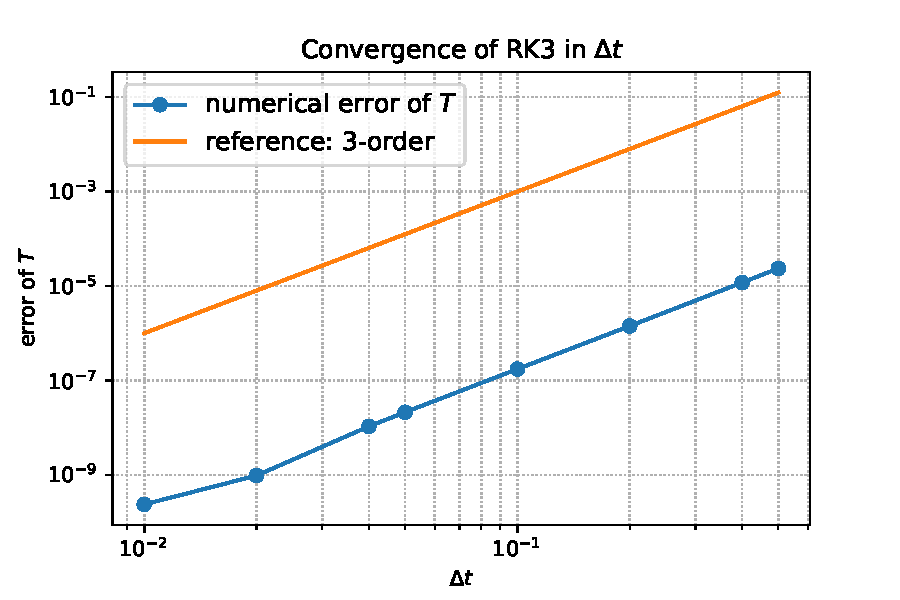
\includegraphics[width = 0.5\linewidth]{dt_2d_bkw_e_full=02}} \hfill
    \subfloat[$e = 0.2$, separate]{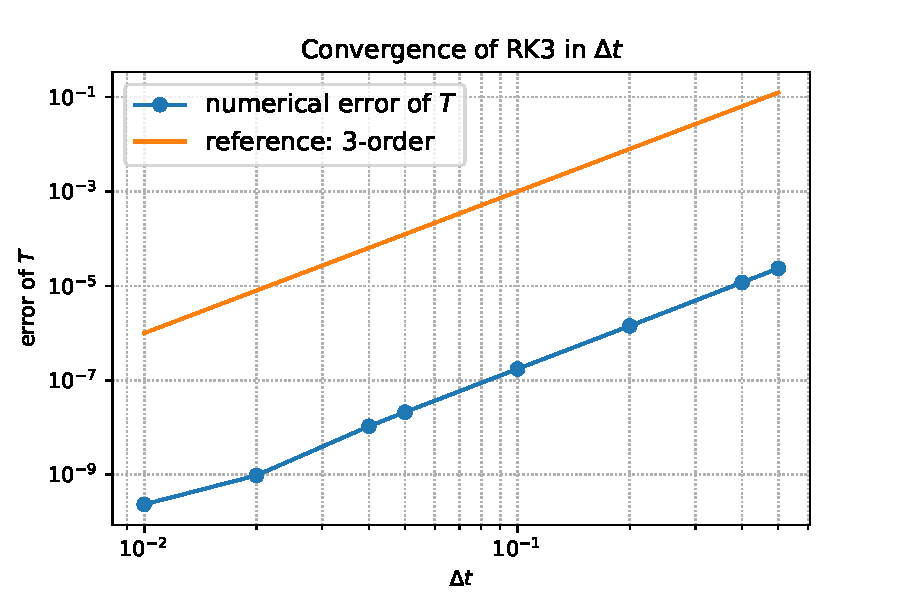
\includegraphics[width = 0.5\linewidth]{dt_2d_bkw_e=02}}\\
   \subfloat[$e = 0.5$, full]{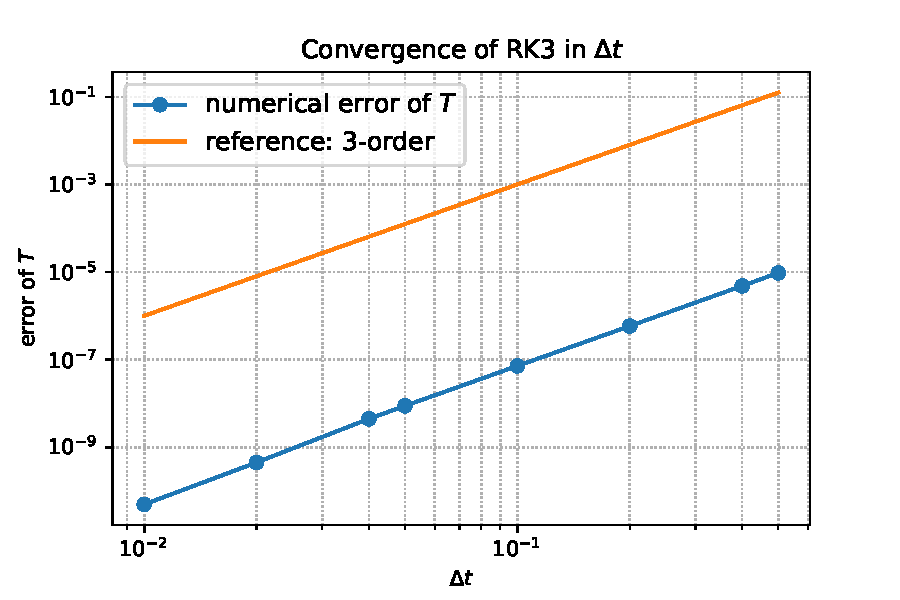
\includegraphics[width = 0.5\linewidth]{dt_2d_bkw_e_full=05}} \hfill
    \subfloat[$e = 0.5$, separate]{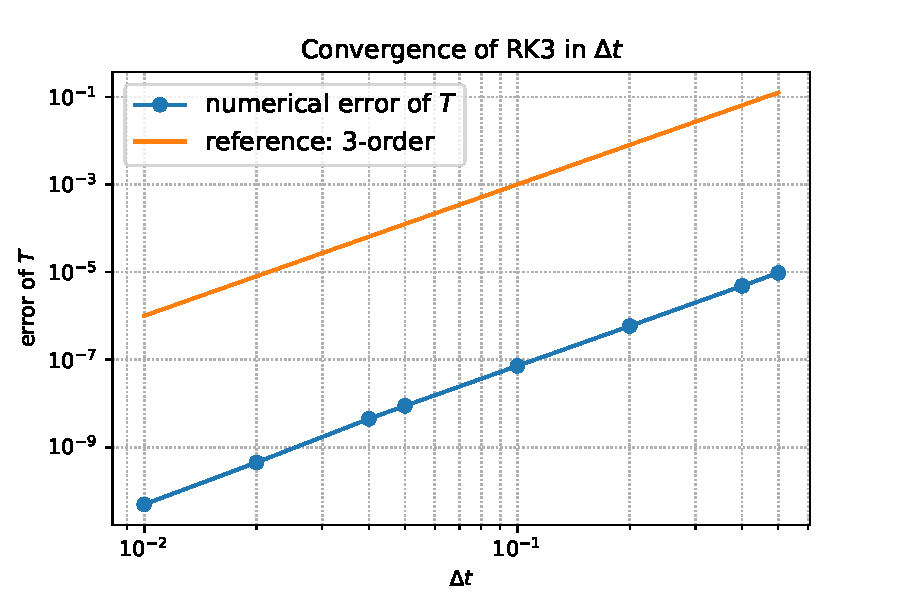
\includegraphics[width = 0.5\linewidth]{dt_2d_bkw_e=05}}\\
  \subfloat[$e = 0.8$, full]{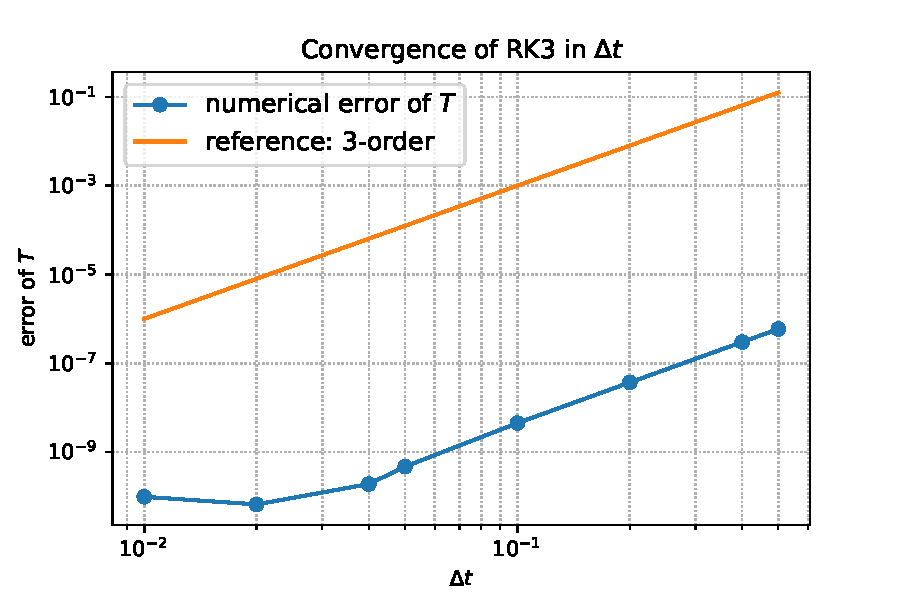
\includegraphics[width = 0.5\linewidth]{dt_2d_bkw_e_full=08}} \hfill
    \subfloat[$e = 0.8$, separate]{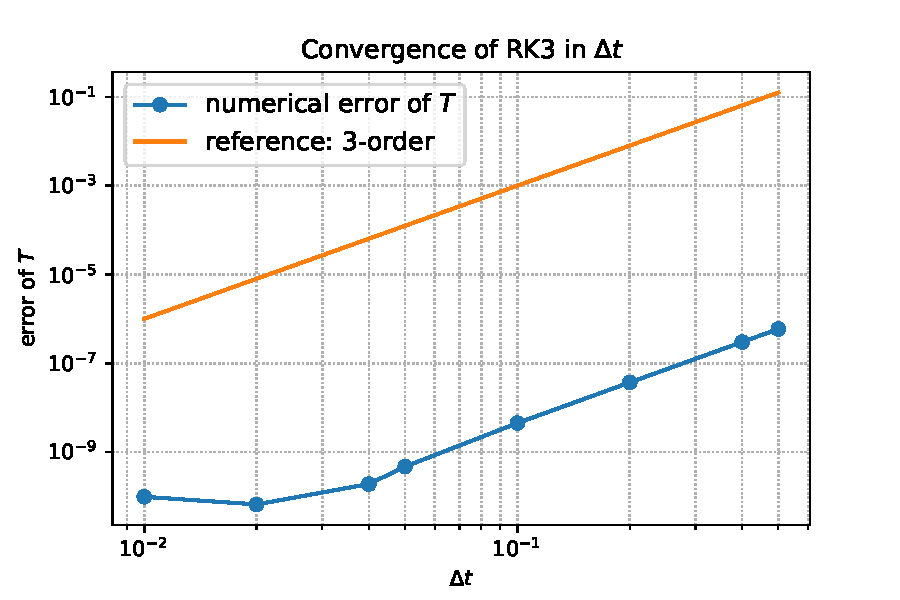
\includegraphics[width = 0.5\linewidth]{dt_2d_bkw_e=08}}
  \caption{Convergence test in time of the 2D Maxwell molecule (isotropic solution) for $e=0.2$, $0.5$ and $0.8$, and for both the ``full" and ``separate" methods. Errors shown here are $|T_\text{num} - T_\text{ref}|$ at $t_\text{final}=2$. $N=64$, $N_{\rho}=30$, $M_{\text{cir}}=30$, $R=7.8$, $L=8.61$.}
  \label{dt_conv_1}
\end{figure}

We then perform the convergence test in $N$. We set $\Delta t = 0.01$ (the previous test suggests that this is sufficient to minimize the time discretization error). In Table~\ref{table 1}, we report the errors for different $N$ at $t_\text{final}=2$. Various values of the restitution coefficient $e = 0.2, 0.5$ and $0.8$, and both the ``full" and ``separate" methods are considered. These results imply that our method can indeed achieve the spectral accuracy, and both the ``full" and ``separate" methods behave similarly for the isotropic solution.

\begin{table}[htp!]
  \centering
  \subfloat[$e = 0.2$]{
  \begin{tabu} to 0.6\linewidth {X[1, c] X[3, c] X[3, c]}
    \toprule
    $N$ &  full & separate  \\
    \midrule
    8  & 9.21116565e-01& 9.21116565e-01 \\
    16 & 1.27640374e-02 & 1.27634481e-02  \\
    32  & 6.79745658e-06 & 6.79544555e-06 \\
    64  & 2.36438646e-10 & 2.34851361e-10 \\
    128  & 6.13890050e-11 & 6.30565600e-11 \\
    \bottomrule
  \end{tabu}
  } \\
  \subfloat[$e = 0.5$]{
  \begin{tabu} to 0.6\linewidth {X[1, c] X[3, c] X[3, c]}
    \toprule
    $N$ & full & separate  \\
    \midrule
    8  & 7.98706096e-01 & 7.98706096e-01 \\
    16  & 6.42644165e-03 & 6.42641236e-03 \\
    32  & 4.55730861e-06 & 4.55713801e-06 \\
    64  & 4.93770580e-11 & 4.93595165e-11 \\
    128  & 3.14279713e-11 & 3.13873372e-11 \\
    \bottomrule
  \end{tabu}
  } \\
  \subfloat[$e = 0.8$]{
  \begin{tabu} to 0.6\linewidth {X[1, c] X[3, c] X[3, c]}
    \toprule
    $N$  & full & separate\\
    \midrule
    8  & 5.52666966e-01 & 5.52666966e-01\\
    16  & 4.88586534e-04 & 4.88821204e-04 \\
    32  & 1.13897201e-07  & 1.14430393e-07\\
    64  & 9.82520731e-11 & 9.82359749e-11 \\
    128 & 1.00117470e-10  & 1.00099595e-10 \\
    \bottomrule
  \end{tabu}
  }
  \caption{Convergence test in $N$ of the 2D Maxwell molecule (isotropic solution) for $e=0.2$, $0.5$ and $0.8$, and for both the ``full" and ``separate" methods. Errors shown here are $|T_\text{num} - T_\text{ref}|$ at $t_\text{final}=2$. $\Delta t = 0.01$, $N_{\rho}=30$, $M_{\text{cir}}=30$, $R=7.8$, $L=8.61$.}
  \label{table 1}
\end{table}


\subsubsection{2D inelastic Maxwell molecules --- anisotropic solution}

To further test the performance of the ``full" and ``separate" methods, we consider the following double-well initial condition
\begin{equation}
  f_0(v) = \frac{0.8}{\pi}\left(\exp(-4|v-2|^2) + \exp(-|v+0.5|^2)\right).
\end{equation}
This function is anisotropic, and $\rho_0=1$, $u_0=0$, $T_0=1.425$.

We choose the same set of parameters as in the previous example and perform the convergence test in $N$. The results are shown in Table~\ref{table 2}. Overall, the accuracy degrades a bit compared to the isotropic solution. Surprisingly, the accuracy of the ``separate" method is much better than the ``full" method when $N$ gets bigger. Although it seems more natural to approximate the gain and loss terms together using the weak formulation, these results suggest that one should use the more accurate formula for the loss term when it is available (intuitively, the smoothing property of the gain term \cite{Lions94} alleviates the error introduced by the quadrature; since the loss term does not have this property, the same quadrature can incur more errors, hence a more accurate formula should be used).

\begin{table}[htp!]
  \centering
  \subfloat[$e = 0.2$]{
  \begin{tabu} to 0.6\linewidth {X[1, c] X[3, c] X[3, c]}
    \toprule
    $N$  & full & separate\\
    \midrule
    8  & 1.25303916e-01 & 1.25303916e-01 \\
    16  & 1.42811856e-02 & 1.41601818e-02 \\
    32  & 8.50383206e-05 & 1.21162093e-04 \\
    64  & 5.75217760e-05  & 8.65618628e-08\\
    128  & 5.74603408e-05 & 2.64749862e-08 \\
    \bottomrule
  \end{tabu}
  } \\
  \subfloat[$e = 0.5$]{
  \begin{tabu} to 0.6\linewidth {X[1, c] X[3, c] X[3, c]}
    \toprule
    $N$ & full & separate \\
    \midrule
    8  & 9.06935081e-02 & 9.06935081e-02 \\
    16  & 2.07345865e-02 & 2.06153352e-02 \\
    32  & 7.68575010e-05  & 1.08598123e-04\\
    64  & 4.58166915e-05 & 3.61540865e-08 \\
    128  & 4.57852460e-05 & 4.84827622e-09 \\
    \bottomrule
  \end{tabu}
  } \\
  \subfloat[$e = 0.8$]{
  \begin{tabu} to 0.6\linewidth {X[1, c] X[3, c] X[3, c]}
    \toprule
    $N$  & full & separate\\
    \midrule
    8 & 4.21932177e-02& 4.21932177e-02  \\
    16 & 2.17989934e-02 & 2.19257970e-02  \\
    32 & 1.17000137e-04 & 1.25546782e-04 \\
    64  & 2.42867607e-05  & 1.55334599e-08\\
    128  & 2.42767854e-05 &  5.91159477e-09 \\
    \bottomrule
  \end{tabu}
  }
  \caption{Convergence test in $N$ of the 2D Maxwell molecule (anisotropic solution) for $e=0.2$, $0.5$ and $0.8$, and for both the ``full" and ``separate" methods. Errors shown here are $|T_\text{num} - T_\text{ref}|$ at $t_\text{final}=2$. $\Delta t = 0.01$, $N_{\rho}=30$, $M_{\text{cir}}=30$, $R=8$, $L=8.83$.}
  \label{table 2}
\end{table}


\subsection{3D examples}

In 3D, the quadrature on the sphere can have a rather nontrivial effect. Therefore, we first test the accuracy of spherical design for Maxwell molecules. Using the same example, we also demonstrate the efficiency of our method by comparing it with the direct Fourier spectral method \cite{FPT05}. After this we numerically verify the physical Haff's cooling law for inelastic hard spheres.

Numerical examples in this subsection are generated using the ``separate" method (the loss term is computed as in (\ref{separate3}).

\subsubsection{3D inelastic Maxwell molecules}

Consider the constant collision kernel $B_{\sigma} = \frac{1}{4\pi}$ and the initial condition:
\begin{equation}\label{3Dbkw}
  f_0(v) = \frac{1}{2(2\pi K)^{3/2}}\exp\left(-\frac{v^2}{2K}\right)\left(\frac{5K-3}{K}+\frac{1-K}{K^2}v^2\right),
\end{equation}
where $K = 1 - \exp(-6.5/6)$. Note that $\rho_0=1$, $u_0=0$ and $T_0=1$.

We perform a convergence test in $M_{\text{sph}}$, the number of spherical design quadrature points used on the unit sphere. We set $e=0.2$, $t_\text{final} = 1$, $\Delta t = 0.01$, $N = 32$, and $N_{\rho}=30$. The results are reported in Table~\ref{table 3}. We find that the error does not decrease further when $M_{\text{sph}}$ reaches $32$. This is due to the fact that the measurement we use is the macroscopic quantity $T$ and other sources of errors such as the truncation of the domain and the discretization in $v$ may pollute the solution. In order to see this error more clearly, we compare the result of our method with that obtained from the direct spectral method (without any speedup strategy), see Table~\ref{table 4}.

\begin{table}[htp!]
  \centering
  \begin{tabu} to 0.8\linewidth {X[1,c] X[2,c]}
    \toprule
    $M_{\text{sph}}$ & $|T_\text{num} - T_\text{ref}|$\\
    \midrule
    6 & 0.0013957739849754791 \\
    12 & 9.9706271716293315e-05 \\
    32 & 2.2499901350947482e-06 \\
    48 & 2.4272557155313734e-06 \\
    70 & 2.4703481364962698e-06 \\
    94 & 2.4703481364962698e-06 \\
    120 & 2.453380453903975e-06 \\
    \bottomrule
  \end{tabu}
  \caption{Convergence test in $M_{\text{sph}}$ of the 3D Maxwell molecule for $e=0.2$. Errors shown here are $|T_\text{num} - T_\text{ref}|$ at $t_\text{final}=1$. $\Delta t = 0.01$, $N = 32$, $N_{\rho}=30$, $R=7$, $L=7.72$.}
  \label{table 3}
\end{table}

\begin{table}[htp!]
  \centering
  \begin{tabu} to 0.8\linewidth {X[1,c] X[2,c]}
    \toprule
    $M_{\text{sph}}$ & $|Q_\text{num} - Q_\text{direct}|_{L^{\infty}}$\\
    \midrule
 	6 & 0.00041820767783433107 \\
	12 & 3.1726851245650724e-05 \\
	32 & 6.5752814213618921e-07 \\
	48 & 5.6132233266191489e-07 \\
	70 & 2.6714628356683257e-07 \\
	94 & 1.0508293902503248e-07 \\
	120 & 2.8872928147741922e-08 \\ 
    \bottomrule
  \end{tabu}
  \caption{Convergence test in $M_{\text{sph}}$ of the 3D Maxwell molecule for $e=0.2$. Errors shown here are $|Q_\text{num} - Q_\text{direct}|_{L^{\infty}}$ at $t_\text{final}=1$. $\Delta t = 0.01$, $N = 32$, $N_{\rho}=30$, $R=7$, $L=7.72$.}
  \label{table 4}
\end{table}

To demonstrate the efficiency of our method, we show in Table~\ref{table 5} and Figure~\ref{CPUtime} the average running time of both the fast method and the direct method for one time evaluation of the collision operator, from which we see a significant speedup ($N=64$ of the direct method is left out due to the memory constraint).

\begin{table}[H]
	\centering
  \begin{tabu} to 0.6\linewidth {X[1, c] X[3, c] X[3, c]}
    \toprule
    $N$ & direct & fast \\
    \midrule
    8 & 32.3ms & 17.6ms \\
    16 & 602ms & 140ms \\
    32 & 23.7s & 1.18s \\
    64 & -- & 9.7s \\
    \bottomrule
  \end{tabu}
  	\caption{Average running time per evaluation of the collision operator. Comparison between the direct method and the fast method for various $N$ and fixed $N_{\rho}=30$, $M_{\text{sph}}=32$.}
	\label{table 5}
 \end{table}

\begin{figure}[htp!]
  \centering
  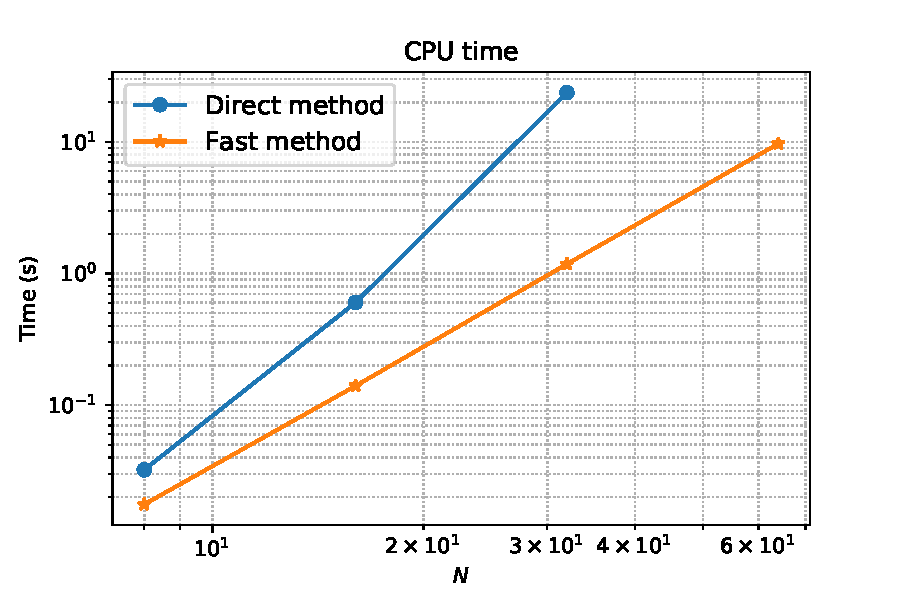
\includegraphics[width = .8\linewidth]{CPU_time}
  \caption{Same numbers as in Table~\ref{table 5} plotted in a log-log scale.}
  \label{CPUtime}
\end{figure}



\subsubsection{3D inelastic hard spheres --- Haff's cooling law}

In this last example, we try to observe the famous Haff's cooling law numerically. First proposed by Haff in 1983 in his seminal work about granular flows \cite{Haff83}, Haff's cooling law implies that the temperature in a spatially homogeneous granular gas composed of inelastic hard spheres decays like $O(t^{-2})$ with time. Note the algebraic decay rather than the exponential decay of Maxwell molecules (cf. (\ref{soln:T})).

We take the same initial data \eqref{3Dbkw} as in the previous example but for hard sphere molecules, that is, consider the collision kernel $B_{\sigma} = \frac{1}{4\pi}|g|$. Also we set $\varepsilon=0$ in equation (\ref{inBoltz}) (the Haff's law is for unheated case, i.e., the homogeneous cooling state). We numerically evaluate the temperature up to time $t_\text{final}=3$ with two different values of restitution coefficient $e=0.2$ and $0.8$. The time evolution of $T$ is shown in Figure~\ref{Haff_cooling}, from which one can see that the numerical temperature decays as 
\begin{equation}
T(t) = \frac{T_0}{(1+C_0 t)^2},
\end{equation}
where the constant $C_0$ depends on the value of $e$. This is in perfect agreement of the Haff's formula (see Section 4.1 of \cite{NE}).

\begin{figure}[htp!]
  \centering
  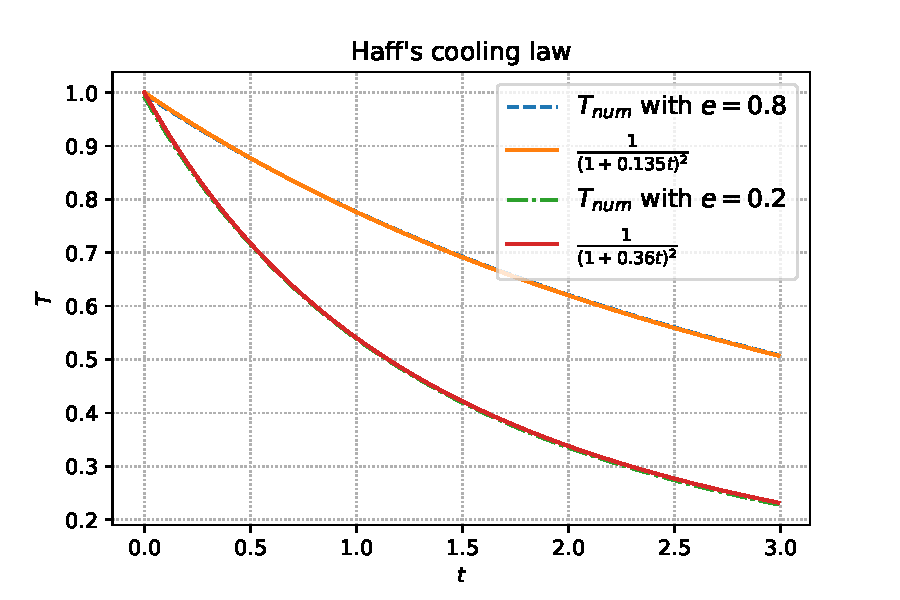
\includegraphics[width = .8\linewidth]{Haff's_cooling}
  \caption{Haff's cooling law. $\Delta t=0.01$, $N=32$, $N_{\rho}=30$, $M_{\text{sph}}=32$, $R=7$, $L=7.72$.}
  \label{Haff_cooling}
\end{figure}


\section{Conclusion}

In this work, we introduced a simple strategy to accelerate the direct Fourier spectral method for the inelastic Boltzmann collision operator, which is an accurate and popular deterministic method for approximating kinetic equations yet has been hindered in real applications due its huge computational cost and memory constraint. Our fast algorithm, by leveraging the low rank and convolutional structure in the collision integral, is able to reduce the computational complexity by orders of magnitude as well as relieve the memory bottleneck in the direct method. A series of numerical experiments has been performed to validate the accuracy and efficiency of the proposed method. In particular, we recovered successfully the Haff's cooling law for inelastic hard spheres. In the future, we will apply the fast solver to the spatially inhomogeneous setting and to simulate more interesting problems in granular materials.




\section*{References}

\bibliography{mybibfile}

\end{document}